\documentclass[a4paper,12pt]{extreport}

%\usepackage{extsizes}
\usepackage{cmap}
\usepackage[utf8]{inputenc} %Кодировка файла 
\usepackage[T2A]{fontenc} %корректное отображение русских шрифтов
\usepackage[english, russian]{babel} %переносы слов
\usepackage{fancyvrb}

%for lcov
\usepackage{lscape} %landspace
\usepackage{float}
\usepackage{tabu}
\usepackage{booktabs}
\usepackage{xcolor}
\definecolor{coverage_Hi}{rgb}{0, 1, 0}
\definecolor{coverage_Med}{rgb}{1, 1, 0}
\definecolor{coverage_Lo}{rgb}{1, 0, 0}
\definecolor{cov_cov}{rgb}{0.9,0.9,1}
\definecolor{cov_diff}{rgb}{1,1,0.5}
\definecolor{cov_nocov}{rgb}{1,0.5,0.5}
\definecolor{cov_nop}{rgb}{0.95,0.95,0.95}
\usepackage{listings}
\usepackage{picture}

\usepackage{graphicx}

%\linespread{1.3}
\renewcommand{\rmdefault}{ftm}
%\frenchspacing

%TimeNewRoman
%\usepackage{fontspec}
%\setmainfont[Mapping=tex-text]{Times New Roman}

%Поля
\usepackage[left=25mm, top=20mm, right=10mm, bottom=20mm, nohead, nofoot]{geometry}

\begin{document}
	\section{Структура проекта}
	
	\section{Тестирование}
		Для тестирования функциональности сервера, было написаны unit-тесты
		с использованием библиотеки cunit. Резултат работы тестиованяи представлен
		в листинге 
		\VerbatimInput{./include/unit_test_out.tex}
		\VerbatimInput{./include/valgrind_out.tex}
		
		Так же было выполнено системное тестирование
		отчет по покрытию тестами представлен в следующей таблице
		\begin{landscape}
			\input{./include/lcov/index}
		\end{landscape}

	\begin{figure}
	\centering
	\includegraphics[width=\textwidth]{./include/smtp_fsm.pdf}
	\caption{Конечный автомат протокола SMTP}
	\label{fig:smtp_fsm}
	\end{figure}

	\begin{figure}
	\centering
	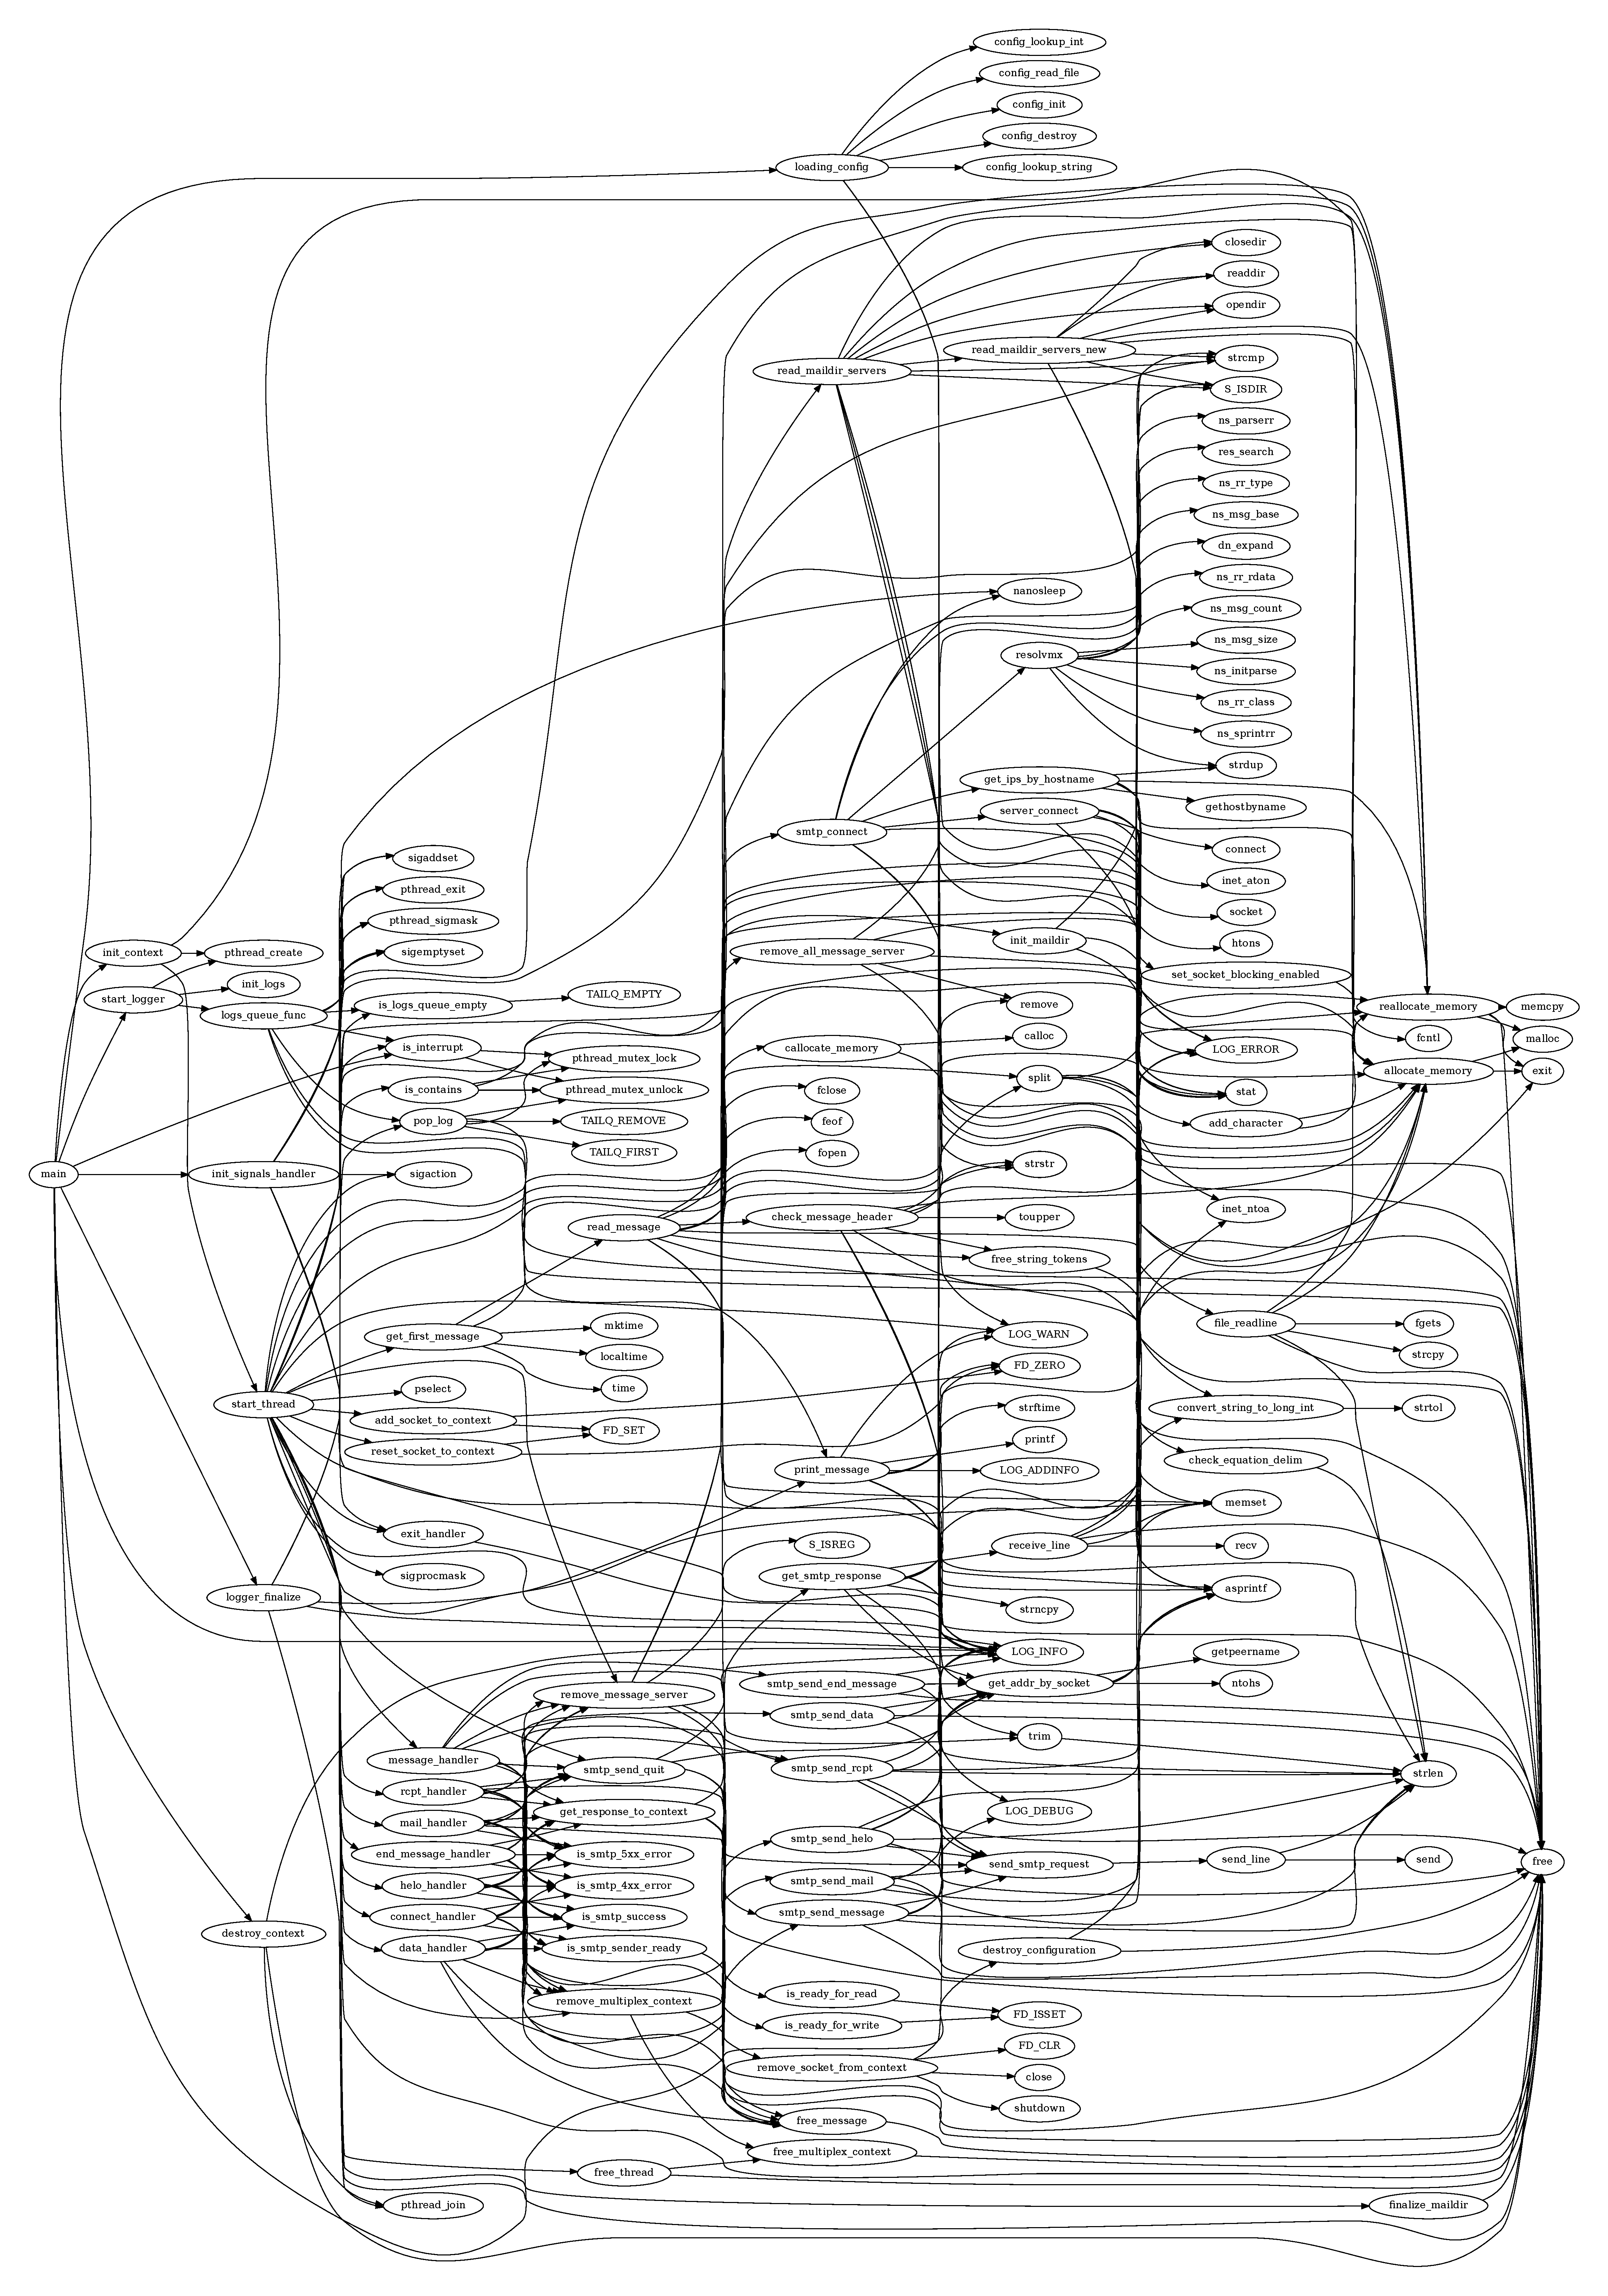
\includegraphics[width=\textwidth]{./include/cflow.pdf}
	\caption{Граф вызовов в модуле EventLoop}
	\label{fig:event}
	\end{figure}


	\section{Список источников и литературы}
	\begin{enumerate}
		\item http://rfc.com.ru/rfc2821.htm
		\item http://rfc.com.ru/rfc1123
		\item https://www.protocols.ru/WP/rfc5322/
	\end{enumerate}
\end{document}